%!TEX program = lualatex
\documentclass[]{beamer}

\usepackage[T1]{fontenc}
\usepackage[slovene]{babel}

\usepackage{amsmath, amsthm, amssymb}

\usepackage[mathrm=sym]{unicode-math}
\setmathfont{Latin Modern Math}

\usepackage{fontspec}
\setsansfont[
  ItalicFont={Fira Sans Light Italic},
  BoldFont={Fira Sans},
  BoldItalicFont={Fira Sans Italic}
]{Fira Sans Light}
\setmonofont[BoldFont={Fira Mono Medium}]{Fira Mono}

\AtBeginEnvironment{tabular}{%
  \addfontfeature{Numbers={Monospaced}}
}

\usepackage[output-decimal-marker={,}]{siunitx}


\usetheme[progressbar=frametitle, block=fill]{moloch}

\graphicspath{ {./slike/} }

\title{Kompleksna eksponentna preslikava in kaos}
% \author[Lenart Miklavič]{Lenart Miklavič\\{\small mentor: doc.~dr.~Uroš Kuzman}}
\subtitle{zagovor diplomske naloge}
\author[Lenart Miklavič]{Lenart Miklavič \and mentor: doc.~dr.~Uroš Kuzman}
\institute[FMF]{Fakulteta za matematiko in fiziko}
\date{27.~avgust 2026}

\theoremstyle{definition}
\newtheorem{definicija}{Definicija}

\theoremstyle{plain}
\newtheorem{izrek}{Izrek}

\begin{document}

\maketitle

\section{Dinamični sistemi}

\begin{frame}
  \frametitle{Diskretni dinamični sistemi}

  Naj bo \(X\) množica, \(x_0 \in X\) element in \(f \colon X \to X\) preslikava.

  \[x_n = f (x_{n - 1})\]

  Ali drugače:

  \[x_0, \quad f (x_0), \quad f (f (x_0)), \quad \ldots\]


\end{frame}


\begin{frame}
  \frametitle{Osnovni pojmi}

  \begin{block}{zaporedje iteracij}
    \centering \(\displaystyle f^0 = \operatorname{Id}, \quad f^{n + 1} = f \circ f^n\)
  \end{block}
  \begin{block}{orbita točke \(x_0 \in X\)}
    \centering \(\displaystyle \big\{ f^n (x_0) \big\}_{n \in \mathbb{N}}\)
  \end{block}
  \begin{block}{periodična točka}
    \centering \(\exists n \in \mathbb{N}. \quad f^n (x_0) = x_0\)
  \end{block}
  \begin{block}{fiksna točka}
    \centering \(f (x_0) = x_0\)
  \end{block}

\end{frame}

\begin{frame}
  \frametitle{Kaos}

  \begin{block}{topološka tranzitivnost}
    \(\forall U, V \text{ odprti}. \quad \exists z_0 \in U. \quad \exists n \in \mathbb{N}: \quad f^n (z_0) \in V\)
  \end{block}

  \begin{block}{občutljivost na začetne pogoje}
    \(\exists \delta > 0. \quad \forall x \in X. \quad \forall U \text{ okolica } x. \quad \exists y \in U. \quad \exists n \in \mathbb{N}:\) \[|f^n (x) - f^n (y)| > \delta\]
  \end{block}


  \pause

  \begin{alertblock}{kaotična preslikava}
    \begin{enumerate}
      \item goste periodične točke
      \item topološka tranzitivnost
      \item občutljivost na začetne pogoje
    \end{enumerate}
  \end{alertblock}

\end{frame}

\begin{frame}
  \frametitle{Robert L.~Devaney}

  \textit{An Introduction to Chaotic Dynamical Systems} (1987)

  \vspace{1cm}

  \centering
  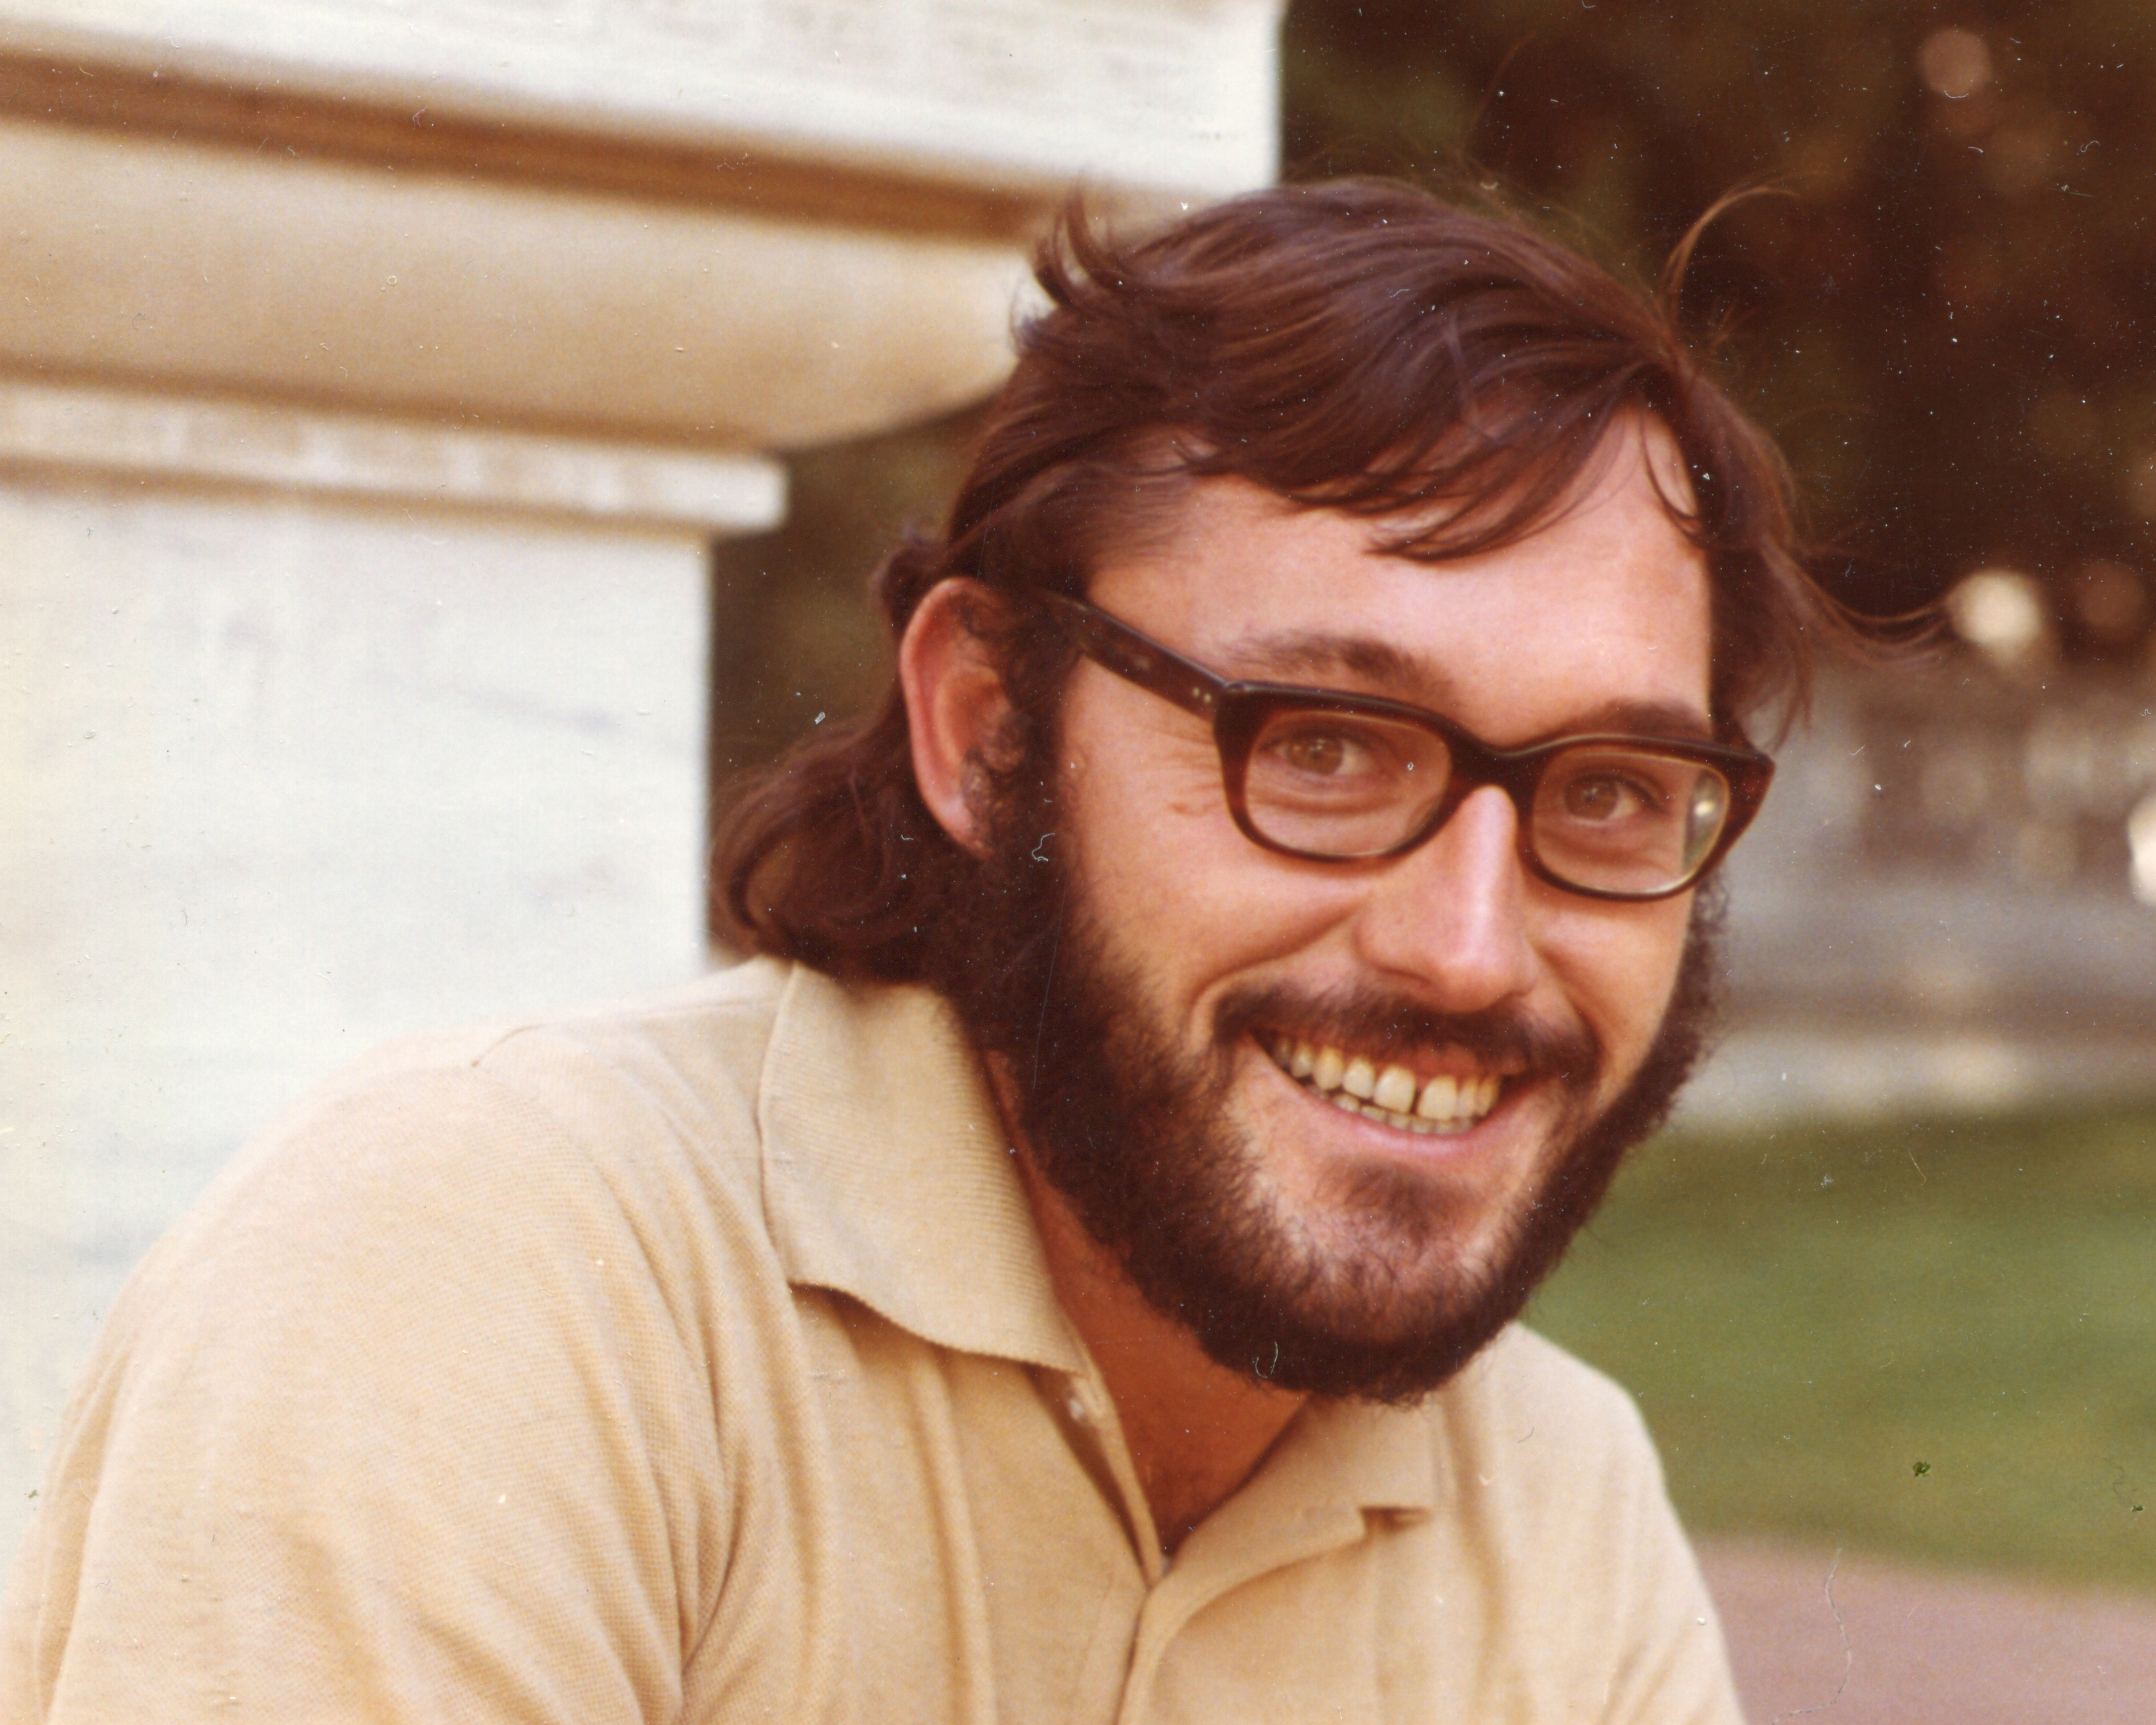
\includegraphics[width=0.6\textwidth]{devaney.jpeg}

\end{frame}

% \begin{frame}
%   \frametitle{Primer}

%   Izberemo poljuben \(x \in \RR\) \pause

%   \begin{itemize}
%     \item Kaj se zgodi, če iteriramo funkcijo \(\sin\)? \pause
%     \item Kaj, če iteriramo funkcijo \(\cos\)? \pause
%     \item Kaj se zgodi, če iteriramo eksponentno funkcijo \(e^x\)? \pause
%           \begin{itemize}
%             \item za \(x \in \CC\)?
%           \end{itemize}
%   \end{itemize}
% \end{frame}

\begin{frame}
  \frametitle{Glavni izrek}

  \begin{itemize}
    \item \(\sin \colon \mathbb{R} \to \mathbb{R}\) \pause
    \item \(\exp \colon \mathbb{R} \to \mathbb{R}\) \pause
    \item \(\exp \colon \mathbb{C} \to \mathbb{C}\)? \pause
  \end{itemize}

  \vspace{0.7cm}

  \centering
  \fbox{
\includegraphics[width=0.9\textwidth]{izrek.pdf}}

\end{frame}

\begin{frame}

  \begin{columns}
    \column{0.5\textwidth}
    \centering
    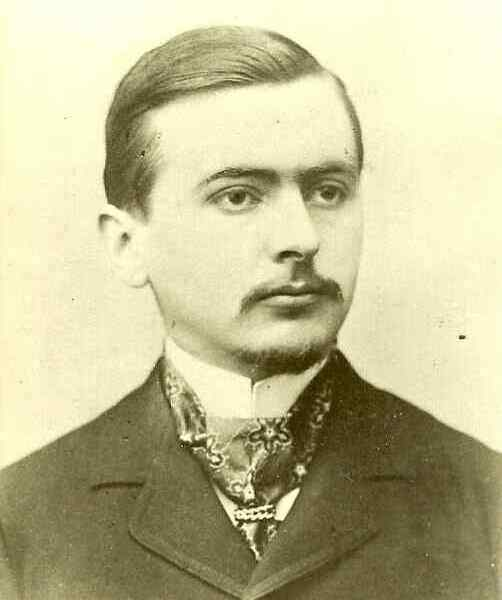
\includegraphics[width=\textwidth]{fatou.jpg}
    \par Pierre Joseph Louis Fatou
    \column{0.5\textwidth}
    \centering
    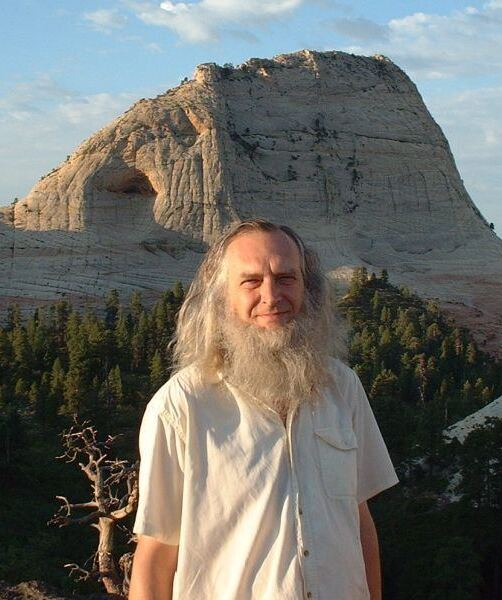
\includegraphics[width=\textwidth]{mihael.jpg}
    \par Michał Misiurewicz
  \end{columns}

\end{frame}

\begin{frame}
  \frametitle{Dokaz}

  \begin{block}{Pickov izrek}
    Naj bosta \(U, V \subsetneq \mathbb{C}\) enostavno povezani območji in \(f \colon U \to V\) holomorfna preslikava. Potem na \(U\) obstaja enolično določena gostota hiperbolične metrike \(\rho_U\), da veljajo naslednje izjave.
    \begin{enumerate}
      \item Za vsak \(z \in \mathbb{D}\) velja \(\rho_{\mathbb{D}} (z) = \frac{2}{1 - |z|^2}\).
      \item Preslikava \(f\) ne veča \emph{hiperboličnega odvoda}, to pomeni, da velja \[\|f (z)\|_{U}^{V} \coloneq |f' (z)| \cdot \frac{\rho_V (f (z))}{\rho_U (z)} \leq 1.\]
      \item Enakost \(\|f (z)\|_{U}^{V} = 1\) velja natanko tedaj, ko je \(f\) biholomorfna.
      \item Če je \(U \subsetneq V\), potem za vsak \(z \in U\) velja \(\rho_U (z) > \rho_V (z)\).
    \end{enumerate}
  \end{block}

\end{frame}

\begin{frame}
  \frametitle{Topološka tranzitivnost}

  \centering
  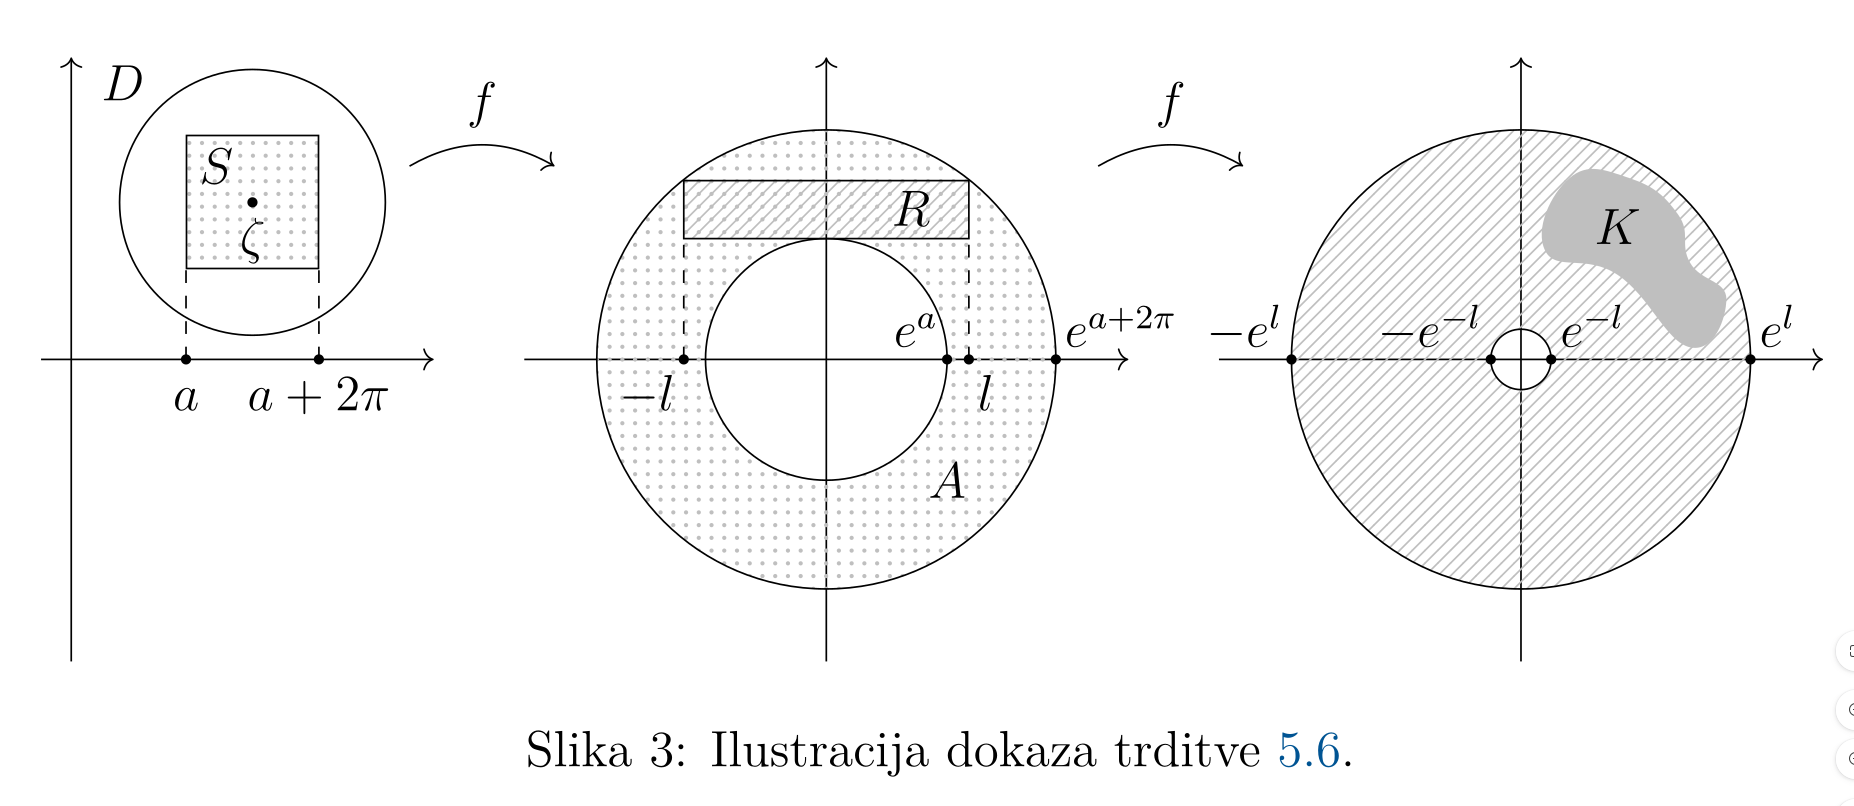
\includegraphics[width=\textwidth]{diski.png}

\end{frame}

\section{Kompleksna dinamika}

\begin{frame}

  \begin{block}{enakomerna konvergenca na kompaktih (EPK)}
    \(\forall K \text{ kompaktna}. \quad \forall \varepsilon > 0. \quad \exists n_0 \in \mathbb{N}. \quad \forall n \geq n_0. \quad \forall z \in K:\) \[|f_n (z) - f (z)| < \varepsilon\]
  \end{block}

  \begin{block}{normalna družina}
    vsako zaporedje ima EPK-konvergentno podzaporedje
  \end{block}

\end{frame}

\begin{frame}

  \begin{block}{Fatoujeva množica \(F (f)\)}
    množica točk z okolico, na kateri je zaporedje iteracij normalno
  \end{block}

  \begin{block}{Juliajeva množica \(J (f)\)}
    \centering \(J (f) = \mathbb{C} \setminus F (f)\)
  \end{block}

\end{frame}

% { % all template changes are local to this group.
%   \setbeamertemplate{navigation symbols}{}
%   \begin{frame}<article:0>[plain]
%     \begin{tikzpicture}[remember picture,overlay]
%       \node[at=(current page.center)] {
%         
\includegraphics[
%           width=\paperwidth,
%           height=\paperheight]{./slike/julia-img0.png}
%       };
%     \end{tikzpicture}
%   \end{frame}
% }

\begin{frame}<article:0>[plain]

  \begin{tikzpicture}[remember picture, overlay]
    \node[at=(current page.center)] {
\includegraphics[height=\paperheight, width=\paperwidth]{julia-img0.png}};
  \end{tikzpicture}

\end{frame}

\begin{frame}[standout]

  Hvala za pozornost!

\end{frame}

\end{document}